\clearpage
\section{The Multi-Axial Atomicity Framework}
\label{sec:atomicity}

The core of Layer~1 is the \emph{multi-axial atomicity} framework: an observable is certified as atomic only if it is simultaneously recognized as such by four independent mathematical frameworks. Convergence across these frameworks provides robustness against the limitations of any single formalism. The \texttt{MetaSpecification} associated with each observable encodes the weighting of these frameworks and defines the ontological grammar of the layer.

\subsection{The Four Primary Decomposition Operators}

Each framework is operationalized by a \emph{decomposition operator} $\decomp_f: \Obs \to \mathcal{P}(\Obs)$, which attempts to decompose an observable into constituent parts. An observable $o$ is \emph{atomic} with respect to framework $f$ if $\decomp_f(o) = \{o\}$ (i.e., no non-trivial decomposition exists).\footnote{In the original architectural specification, decomposition operators are denoted by $\Delta_f$, with $f \in \{\mathrm{bool}, \mathrm{measure}, \mathrm{cat}, \mathrm{info}\}$. We retain this notation here for formal consistency. The implementation uses the class name \texttt{DecompositionOperator} with a registry of framework-specific functions.}

\paragraph{Boolean Atomicity (Proposition~A.1).}
In a Boolean algebra $\mathcal{B}$, an element $a \neq 0$ is an atom if there exists no $b$ such that $0 < b < a$. The \texttt{BooleanDecompositionOperator} implements this for discrete values: for sets, the partial order is induced by inclusion; for integers, by divisibility. The operator returns a decomposition into a minimal non-empty subset and its complement if one exists; otherwise, the observable is Boolean-atomic.

\begin{lstlisting}[language=Python, caption={Boolean atomicity test for the integer 1}, label={lst:boolean}]
>>> from apeiron.layer01 import boolean_atomicity
>>> obs = UltimateObservable(id="one", value=1, observability_type=ObservabilityType.DISCRETE)
>>> boolean_atomicity(obs)
1.0
\end{lstlisting}

\paragraph{Measure-Theoretic Atomicity (Proposition~A.2).}
Given a measure space $(\Omega, \Sigma, \mu)$, a set $A \in \Sigma$ with $\mu(A) > 0$ is an atom if for every measurable $B \subseteq A$, either $\mu(B) = 0$ or $\mu(B) = \mu(A)$. The \texttt{MeasureDecompositionOperator} approximates this by sampling subsets and checking measure invariance. For efficiency, the implementation restricts exhaustive enumeration to sets of size $\le 20$; for larger sets, random sampling with a configurable limit is used.

\paragraph{Categorical Atomicity (Proposition~A.3).}
In a category $\mathcal{C}$ with a zero object $0$, an object $X$ is \emph{simple} if it is isomorphic to a zero object. The \texttt{CategoricalDecompositionOperator} attempts to factor $o$ as a product/coproduct of non-trivial objects; if no such factorization exists, $o$ is categorically atomic. The operator also checks whether the object satisfies the zero-object property (simultaneously initial and terminal).

\paragraph{Information-Theoretic Atomicity (Proposition~A.4).}
An observable $o$ is information-theoretically atomic if its Kolmogorov complexity $K(o) \ge |o| - c$, i.e., it is algorithmically random and therefore incompressible. The \texttt{InformationDecompositionOperator} uses zlib compression as a computable proxy. For a string $s$, if $|zlib(s)| \ge |s| - c$, the string is considered incompressible and thus atomic. The operator also detects homogeneous blocks (e.g., \texttt{"aaabbb"}) and splits them when the combined complexity of the parts is lower than that of the whole.

% ---------- Radar Chart voor Apeiron Space ----------
\begin{figure}[htbp]
\centering
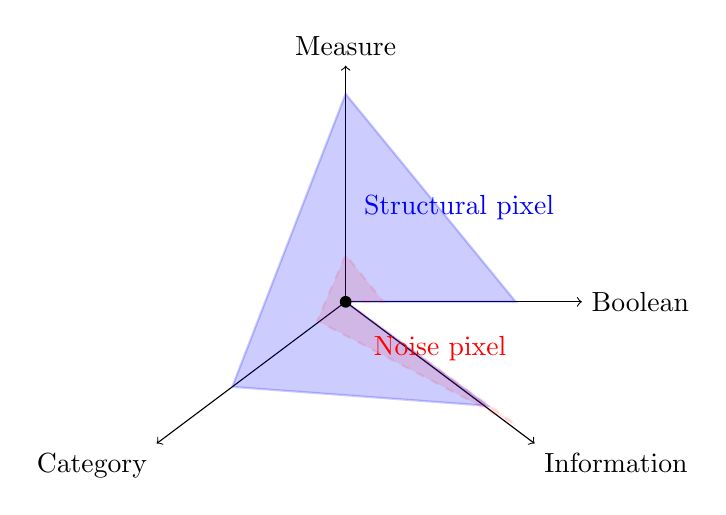
\begin{tikzpicture}[scale=1.2]
    % Assen
    \draw[->] (0,0) -- (2.5,0) node[right] {Boolean};
    \draw[->] (0,0) -- (0,2.5) node[above] {Measure};
    \draw[->] (0,0) -- (-2.0,-1.5) node[below left] {Category};
    \draw[->] (0,0) -- (2.0,-1.5) node[below right] {Information};
    
    % Voorbeeld 1: structurele pixel (hoog op alle assen)
    \draw[blue, thick, fill=blue, opacity=0.2] (0,0) -- (1.8,0) -- (0,2.2) -- (-1.2,-0.9) -- (1.5,-1.1) -- cycle;
    \node[blue] at (1.2,1.0) {Structural pixel};
    
    % Voorbeeld 2: ruis pixel (laag op Boolean/Measure, hoog op Info)
    \draw[red, thick, dashed, fill=red, opacity=0.1] (0,0) -- (0.4,0) -- (0,0.5) -- (-0.3,-0.2) -- (1.8,-1.3) -- cycle;
    \node[red] at (1.0,-0.5) {Noise pixel};
    
    \node at (0,0) [circle, fill=black, inner sep=1.5pt] {};
\end{tikzpicture}
\caption{Schematic radar chart of the four atomicity axes. A structural pixel (e.g., on a digit stroke) scores high on Boolean, Measure, and Category axes, while a noise pixel exhibits high Information atomicity (incompressibility) but low structural coherence. The actual scores are computed continuously and weighted via the MetaSpecification.}
\label{fig:radar}
\end{figure}
% ----------------------------------------------------

\subsection{The Apeiron Space: A Categorical Perspective}
\label{sec:apeiron_space}

The four decomposition axes can be unified in a categorical framework. Let $\mathcal{A}$ be the \emph{Apeiron category} whose objects are observables $o \in \Obs$ and whose morphisms are generated by the decomposition operators $\decomp_f$. The multi-axial atomicity condition then states that $o$ is \emph{atomic} if it is a \emph{zero object} in the full subcategory spanned by the four frameworks---i.e., it is simultaneously initial and terminal with respect to each decomposition functor.

\begin{figure}[htbp]
\centering
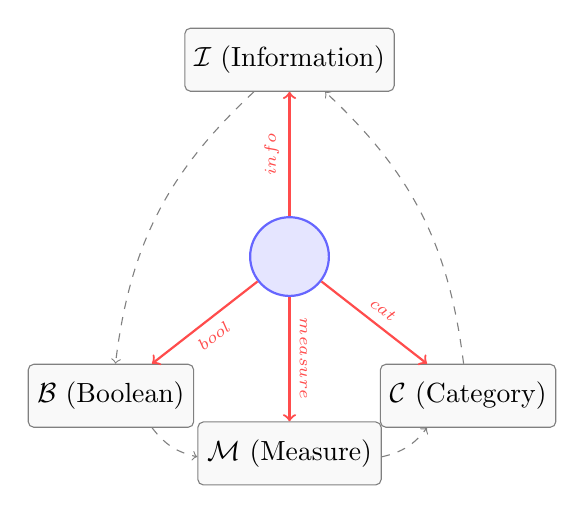
\begin{tikzpicture}[node distance=2.5cm, auto,
    atom/.style={circle, draw=blue!60, fill=blue!10, thick, minimum size=1cm},
    axis/.style={rectangle, draw=gray, fill=gray!5, rounded corners=2pt, minimum width=1.8cm, minimum height=0.8cm}]
    
    \node[atom] (O) {$\Obs$};
    \node[axis] (B) [below left of=O, xshift=-0.5cm] {$\mathcal{B}$ (Boolean)};
    \node[axis] (M) [below of=O] {$\mathcal{M}$ (Measure)};
    \node[axis] (C) [below right of=O, xshift=0.5cm] {$\mathcal{C}$ (Category)};
    \node[axis] (I) [above of=O] {$\mathcal{I}$ (Information)};
    
    \draw[->, red!70, thick] (O) -- node[swap, sloped, font=\footnotesize] {$\decomp_{\text{bool}}$} (B);
    \draw[->, red!70, thick] (O) -- node[sloped, font=\footnotesize] {$\decomp_{\text{measure}}$} (M);
    \draw[->, red!70, thick] (O) -- node[sloped, font=\footnotesize] {$\decomp_{\text{cat}}$} (C);
    \draw[->, red!70, thick] (O) -- node[sloped, font=\footnotesize] {$\decomp_{\text{info}}$} (I);
    
    \draw[dashed, ->, gray] (B) to [bend right=20] (M);
    \draw[dashed, ->, gray] (M) to [bend right=20] (C);
    \draw[dashed, ->, gray] (C) to [bend right=20] (I);
    \draw[dashed, ->, gray] (I) to [bend right=20] (B);
\end{tikzpicture}
\caption{Commutative projection of an observable onto the four atomicity axes. Atomicity holds iff the object is preserved (up to isomorphism) by all four projections.}
\label{fig:commutative}
\end{figure}

This categorical lens not only provides formal rigor but also suggests a natural path to Layer~2: the relational hypergraph corresponds to the \emph{nerve} of the category of atomic observables, where higher-dimensional simplices encode multi-way co-occurrences.

\subsection{Atomicity Score and Meta-Specification}

The overall atomicity score $\atomicity(o)$ is a weighted average of the framework-specific binary scores:
\[
\atomicity(o) = \sum_{f \in \{\text{bool}, \text{measure}, \text{cat}, \text{info}\}} \meta.\text{weights}[f] \cdot \mathbf{1}[\decomp_f(o) = \{o\}].
\]
The \texttt{MetaSpecification} class (Listing~\ref{lst:metaspec}) stores the primary principles, the weights, and the axiomatic commitments of the layer. Each \texttt{UltimateObservable} holds a copy of its \texttt{MetaSpecification}, ensuring that observer-relative atomicity judgments are isolated and reproducible.

\begin{lstlisting}[language=Python, caption={The \texttt{MetaSpecification} class (excerpt)}, label={lst:metaspec}]
@dataclass
class MetaSpecification:
    primary_principles: List[DecompositionPrinciple]
    atomicity_is_binary: bool = False
    default_atomicity_weights: Dict[str, float] = field(default_factory=...)
    qualitative_dim_weights: Dict[str, float] = field(default_factory=dict)
    axioms: List[str] = field(default_factory=lambda: [
        "irreducibility_is_observer_relative",
        "atomicity_is_continuous_not_binary",
        "decomposition_vacuity_implies_atomicity",
        "generativity_requires_non_null_resonance",
    ])
\end{lstlisting}

\subsection{Qualitative Dimensions and Relational Context}

Beyond the four primary frameworks, Layer~1 supports \emph{qualitative dimensions}—intrinsic properties such as intensity, density, colour, and texture. Each dimension is itself subject to atomicity testing via the \texttt{QualitativeDecompositionOperator}. The \texttt{DensityField} class (Listing~\ref{lst:density}) captures the relational influence among observables through a two-channel model (resonance + embedding), enabling the system to compute influence matrices and perform Monte Carlo sampling of influence distributions.

\begin{lstlisting}[language=Python, caption={The \texttt{DensityField} influence model}, label={lst:density}]
def _compute_pairwise_influence(self, target, target_emb, other):
    similarity = cosine(target_emb, other.relational_embedding)
    distance = 1 - similarity
    resonance = decay * w_target * w_other / (1 + distance)
    embedding = decay * max(0, similarity)
    return resonance_channel_weight * resonance + embedding_channel_weight * embedding
\end{lstlisting}